\newlength{\bibsep}
\documentclass[nonatbib,5p,a4paper]{elsarticle}  % 5p for two columns, 1p for 1 column (this is specific for the elsearticle)
\usepackage[italian,norsk,nynorsk]{babel}        % Language
\usepackage[DatePublished]{Code/NTNU-lab}        % remove [DatePublished] to remove dates
\usepackage{csquotes}                            % Must be loaded when babel is loaded to avoid error.
% Use this file to write code that you do not want in the .sty file, but has to be in the preamble (before \begin{document}).
% Writing in this file in stead of in the preamble will keep the main file more organised and tidy.


%                       Nomenclatures
%_______________________________________________________________
\usepackage[intoc]{nomencl}
\makenomenclature

\renewcommand{\nomname}{%
% Title
%----------------
List of Symbols
%----------------
}
\renewcommand{\nompreamble}{%
% Description
%----------------
The next list describes several symbols that will be later used within the body of the document
%----------------
}
% This code creates the groups
\renewcommand\nomgroup[1]{%
  \item[\bfseries
  \ifstrequal{#1}{A}{Physics constants}{%
  \ifstrequal{#1}{B}{Mathematical constants}{%
  \ifstrequal{#1}{C}{Other symbols}{}}}%
]}
% This will add the units
\newcommand{\nomunit}[1]{%
\renewcommand{\nomentryend}{\\#1}}
%................................................................

                            % Write all preamble code in this file to keep it organised and tidy.

\addbibresource{Bibliography/Sources.bib}        % Selects the Bibliography file.


\begin{document}
\selectlanguage{italian}                         % Sets the language of the document.

%%%%%%%%%%%%%%%%%%%%%%%%%%%%%%%%%%%%%%%%

\begin{frontmatter}
%
% Title:
%------------------------------------
\title{Circuiti 3}
%
% Authors:
%------------------------------------
% List an author with name ' Firstname Middlename Lastname ' like this:
% F. M. Lastname
\author{L. Trombetta} 
\author{A. Turturiello}
\author{F. Venturoli}
%
% Date:
%------------------------------------
%
\newdate{dateName}{19}{06}{2022} % edit the date here, ' dateName ' has to match on these two lines.
\renewcommand*{\today}{\MonthYearDateFormat\displaydate{dateName}} 
% Options for displaying date: \MonthYearDateFormat,  \DayMonthYearDateFormat or \YearDateFormat
%
% Abstract:
%------------------------------------

\NameOfAbstract{Abstract}
 % Change abstract title here. If you write in Norwegian, write 'Sammendrag' (nb) or 'Samandrag' (nn)
\begin{abstract}
% Delete the text and write your abstract here:
%------------------------------------

Lo scopo dell'esperienza è stato quello di studiare i circuiti RC, RL e RLC attraverso la nozione di impedenza e, quindi, di funzione di trasferimento in corrente impulsata a onda sinusoidale e delle diverse componenti circuitali.

\end{abstract}
%
\end{frontmatter}
%
%
% Table of contents:
%------------------------------------
% If the report is very long for some reason (over 4 or 5 pages), use a table of contents.
% Uncomment everything below the line ---- to get table of contents (ctrl + /) (the / on numberpad):
%-------------
%
% \ 
 \vspace{1cm}

 \begin{minipage}{\textwidth}
     \tableofcontents
 \end{minipage}
 \clearpage
%% Prints a list of symbols. You can create/ change the categories in the preamble.tex file. 
% Learn more about nomenclature: https://www.overleaf.com/learn/latex/Nomenclatures

\nomenclature[A, 02]{\(c\)}{\href{https://physics.nist.gov/cgi-bin/cuu/Value?c}
{Speed of light in a vacuum}
\nomunit{\SI{299792458}{\meter\per\second}}}
\nomenclature[A, 03]{\(h\)}{\href{https://physics.nist.gov/cgi-bin/cuu/Value?h}
{Planck constant}
\nomunit{\SI[group-digits=false]{6.62607015e-34}{\joule\per\hertz}}}
\nomenclature[A, 01]{\(G\)}{\href{https://physics.nist.gov/cgi-bin/cuu/Value?bg}
{Gravitational constant} 
\nomunit{\SI[group-digits=false]{6.67430e-11}{\meter\cubed\per\kilogram\per\second\squared}}}
\nomenclature[B, 03]{\(\mathbb{R}\)}{Real numbers}
\nomenclature[B, 02]{\(\pi\)}{Pi}
\nomenclature[B, 01]{\(e\)}{Euler's constant}
\nomenclature[C]{\(V\)}{Constant volume}
\nomenclature[C]{\(\rho\)}{Friction index}
\printnomenclature

                 % List of symbols, can be useful
\section{Introduzione e descrizione dell'apparato sperimentale}
Per condurre l'esperienza ci siamo serviti di una Breadboard dotata di due boccole e di una griglia di fori in cui inserire i refori. La griglia è caratterizzata dalla presenza di quattro colonne indicate con i simboli "+" e "-", ciascuna equipotenziale, e altre venti colonne equipotenziali riga per riga, indicate con delle lettere. Lo strumento ci ha permesso di realizzare i circuiti su cui abbiamo condotto le diverse misure. Le componenti di circuito di cui ci siamo serviti sono state le resistenze, di cui abbiamo ricavato i valori tramite un \textit{tool online}\footnote{ https://www.digikey.it/it/resources/conversion-calculators/conversion-calculator-resistor-color-code}, diodi di silicio e un partitore resistivo, composto da boccole e da interruttori in grado di modificare la resistenza dello strumento.
Abbiamo fatto uso di due multimetri, strumenti in grado di misurare diverse grandezze, nel nostro caso utilizzati per determinare la differenza di potenziale tra due punti del circuito e l'intensità di corrente.
Infine, abbiamo collegato un generatore che fornisse corrente ai circuiti, attraverso il controllo della sua differenza di potenziale.

\begin{figure}[h!]
    \centering
    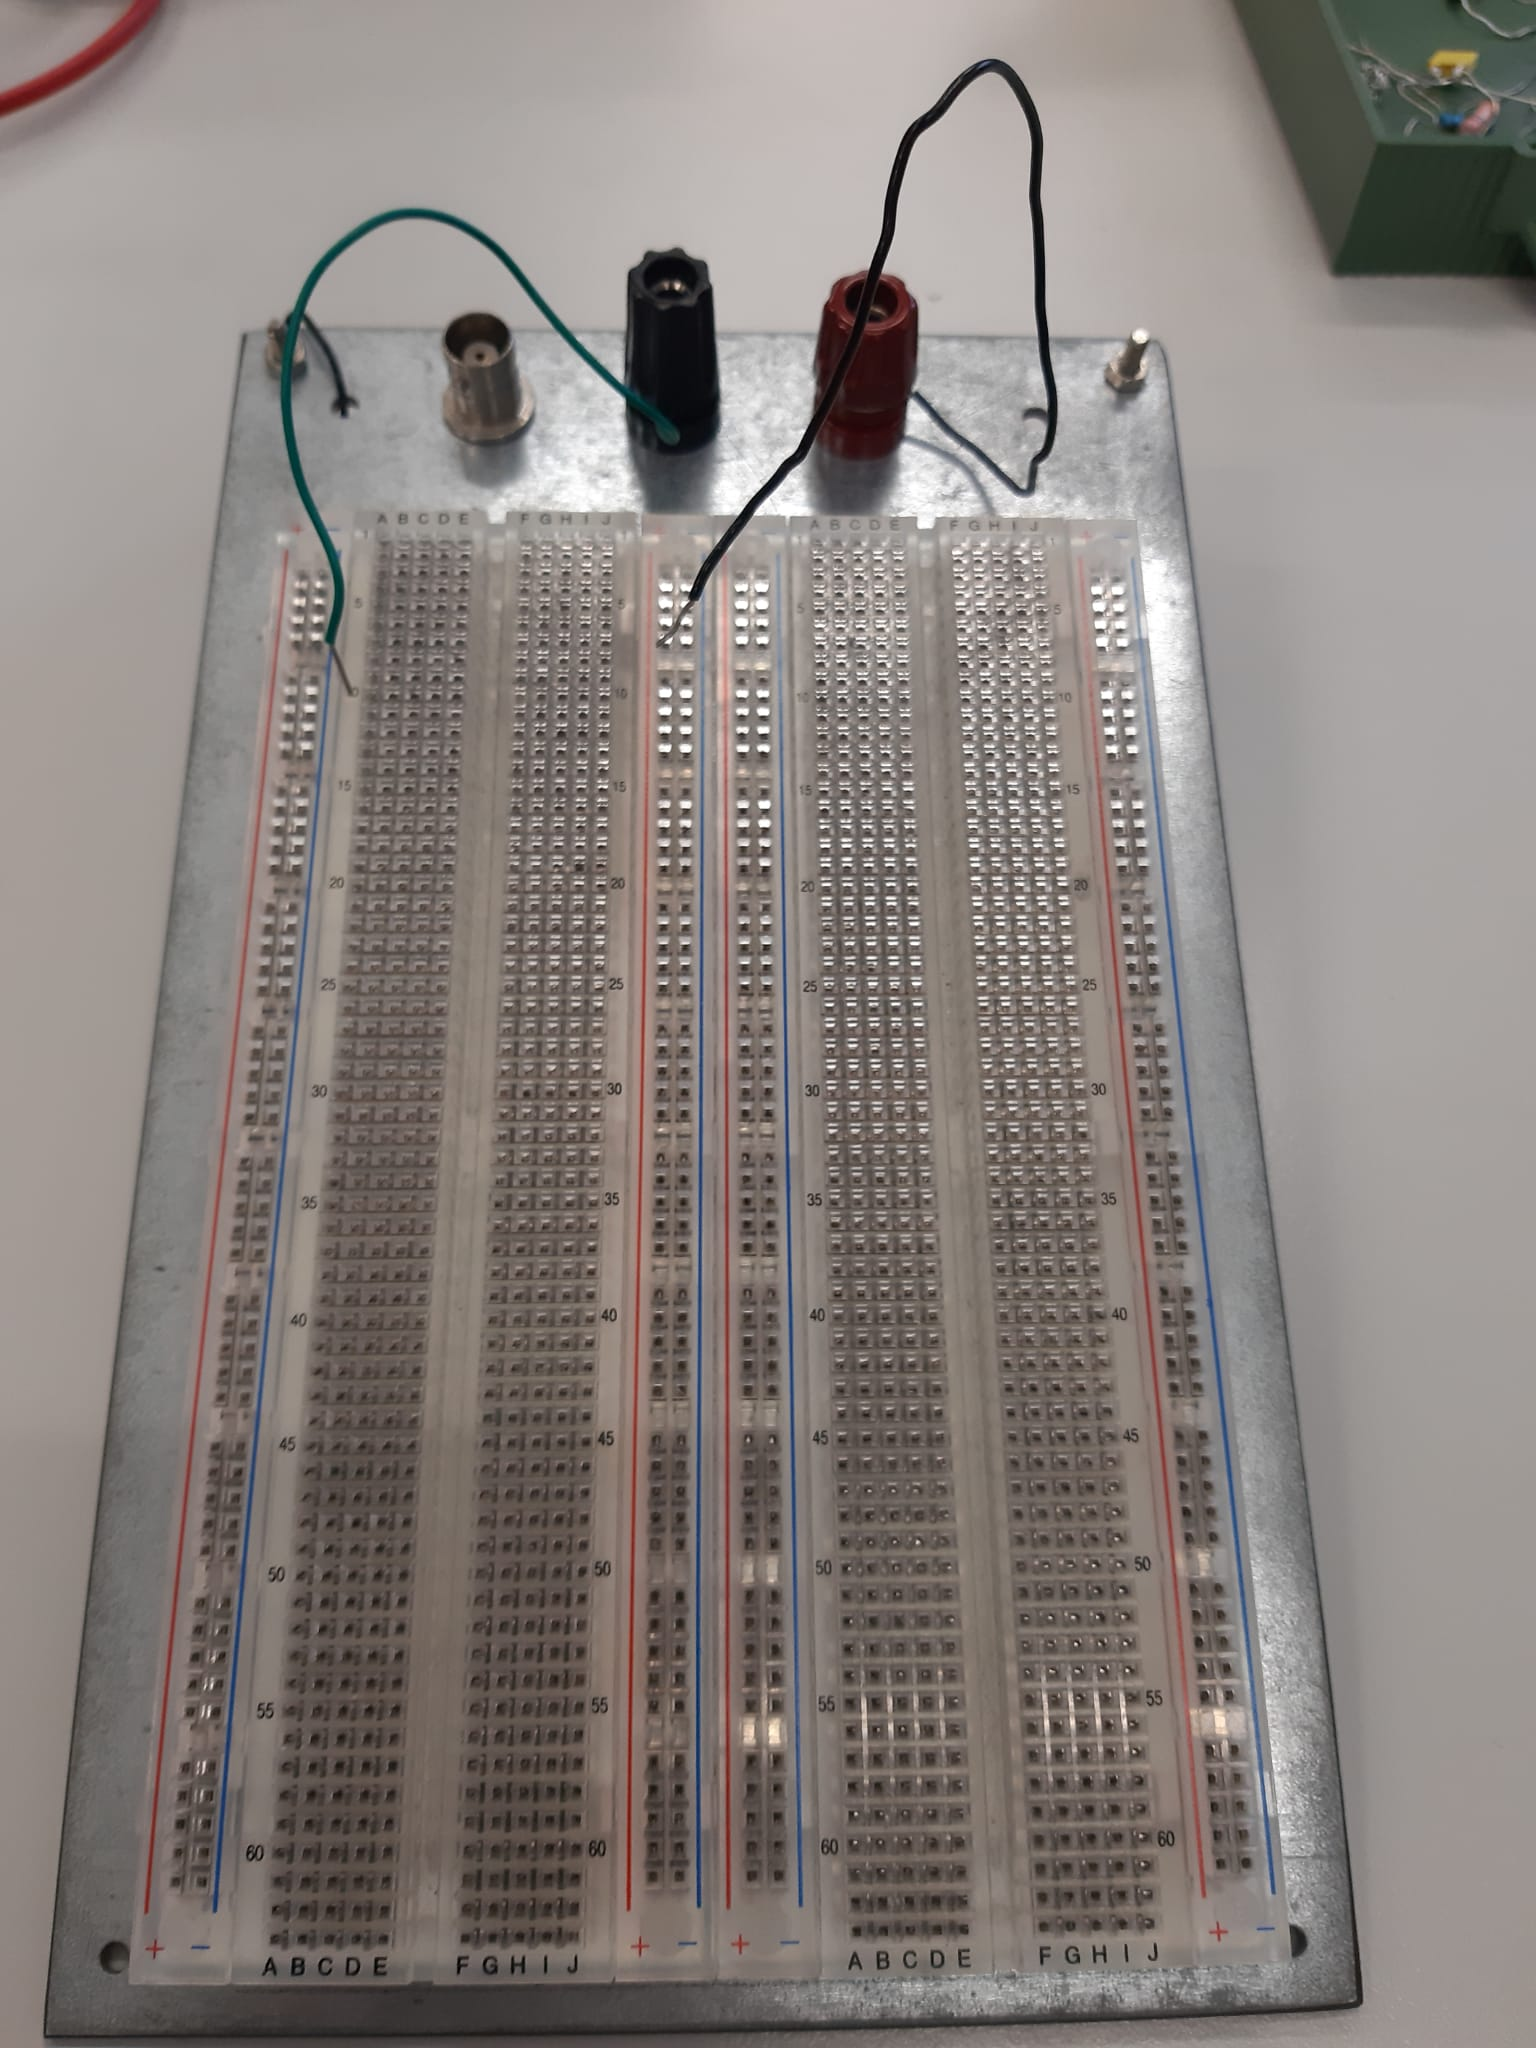
\includegraphics[scale=0.1]{Immagini/Circuitoooo.jpeg}
    \label{fig:my_label}
\end{figure}

La prima parte dell'esperienza si è concentrata sullo studio della strumentazione di laboratorio, studio finalizzato ad utilizzare configurazioni adeguate nelle parti successive. E' stato, infatti, necessario verificare che il multimetro usato come Voltmetro fosse ben progettato, cioè che avesse la caratteristica di possedere una resistenza in parallelo grande. Analogamente, è stato necessario verificare che il multimetro usato come Amperometro avesse la caratteristica di possedere una resistenza in serie piccola.
Successiavmente ci siamo concenrati sullo studio delle resistenze e della Legge di Ohm:

\begin{equation}
\frac{1}{R_{\parallel}}=\sum_{i=1}^{N}\frac{1}{R_{i}} \hspace{73 pt} R_{\perp}=\sum_{i=1}^{N}R_{i}
\end{equation}

\begin{equation}
V=R_{tot}I
\end{equation}

Infine, abbiamo studiato la Legge di Shockley, che descrive l'andamento di corrente per i diodi:

\begin{equation}
I=I_{0}(e^{qv/gK_b T}-1)
\end{equation}

indicando con \textit{q} la carica degli elettroni, con $K_b$ la costante di Boltzmann, con \textit{g} la costante che dipende dal tipo di diodo e con T la temperatura del diodo in Kelvin, corrispondente a quella dell'ambiente. Il termine di proporzionalità $I_0$ è detto \textit{intensità di corrente di saturazione}, il valore che ci aspettiamo di ottenere è molto piccolo in quanto si tratta di una corrente generata dai portatori di carica interni al diodo in diffusione dalla regione neutra alla regione di carica spaziale\footnote{Si tratta di una regione isolante all'interno di un semiconduttore drogato.}.
%% Place large figures that span the whole width of the page in here to easily move them around in the file
% and to avoid getting figures displayed after references and appendix. 
%
% Use {figure*} for a figure that will span both columns. 
% Below is an example of a figure with 6 sub-figures.
\begin{figure*}
%
        \subfigure[Contour plot number 1]{%
            \label{fig:Contour_1}
            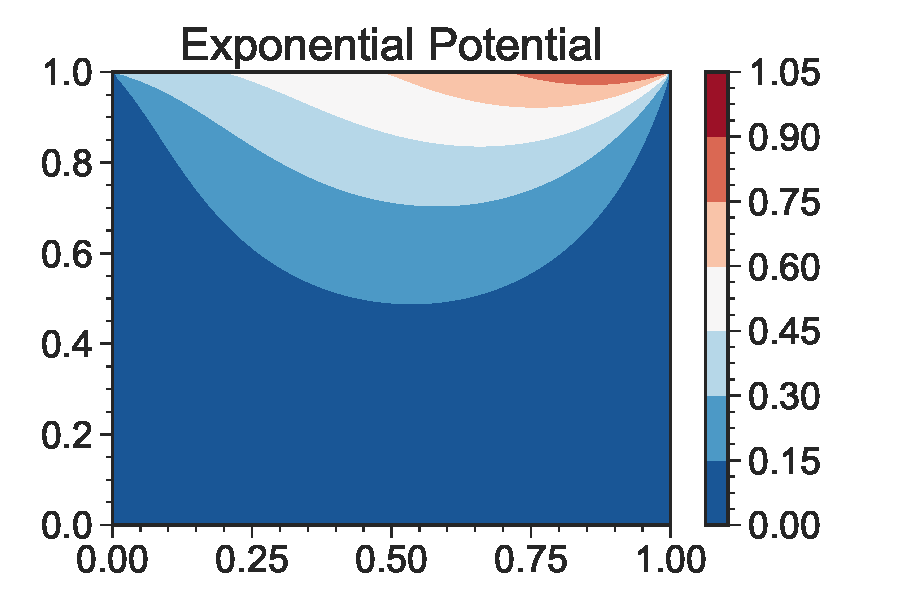
\includegraphics[width=0.3\textwidth]{Images/Fig:Countour-plot/1-contour.pdf}
        }%
        \hspace{1em}
        \subfigure[Contour plot number 2]{%
            \label{fig:Contour_2}
            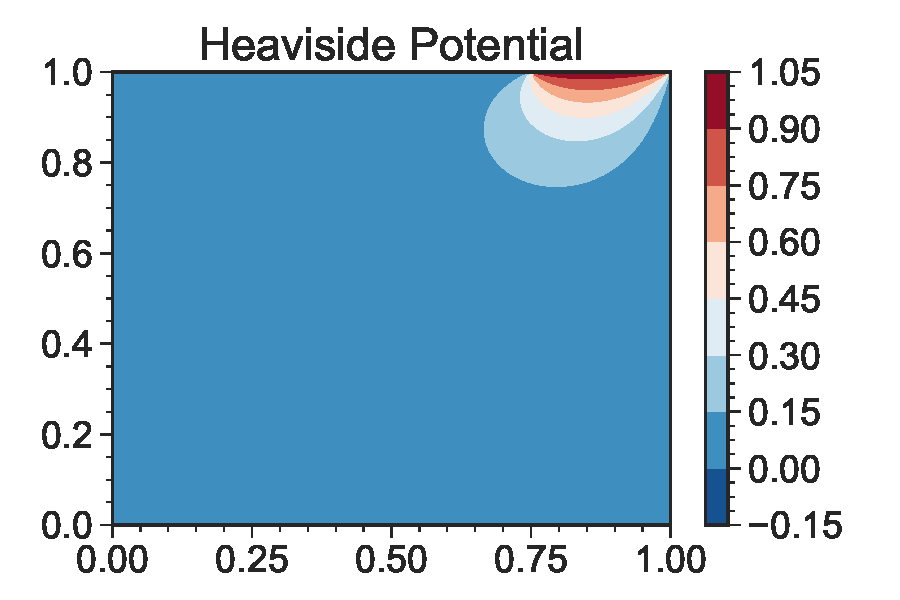
\includegraphics[width=0.3\textwidth]{Images/Fig:Countour-plot/2-contour.pdf}
        }%
        \hspace{1em}
        \subfigure[Contour plot number 3]{%
           \label{fig:Contour_3}
           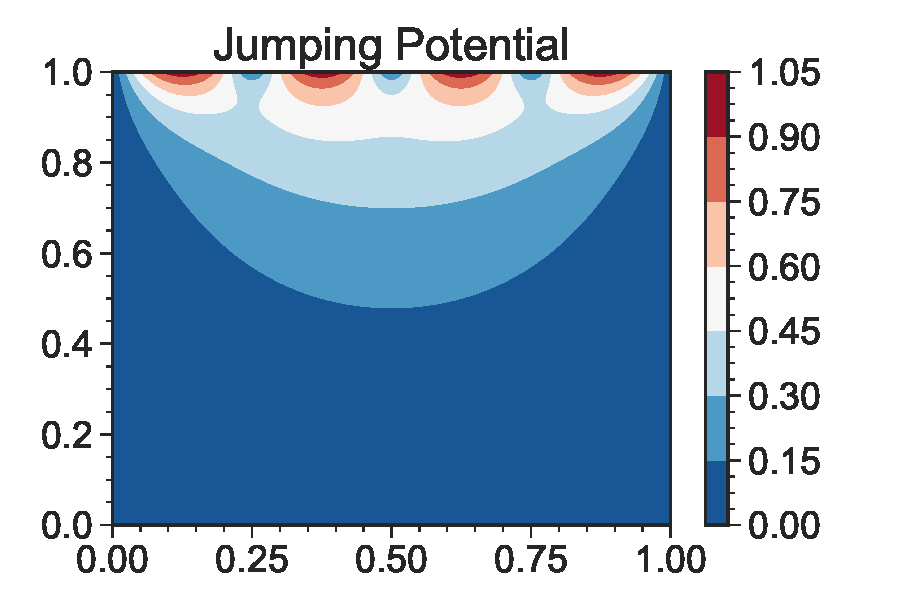
\includegraphics[width=0.3\textwidth]{Images/Fig:Countour-plot/3-contour.pdf}
        }\\ %  ------- End of the first row ----------------------%
        \subfigure[Contour plot number 4]{%
            \label{fig:Contour_4}
            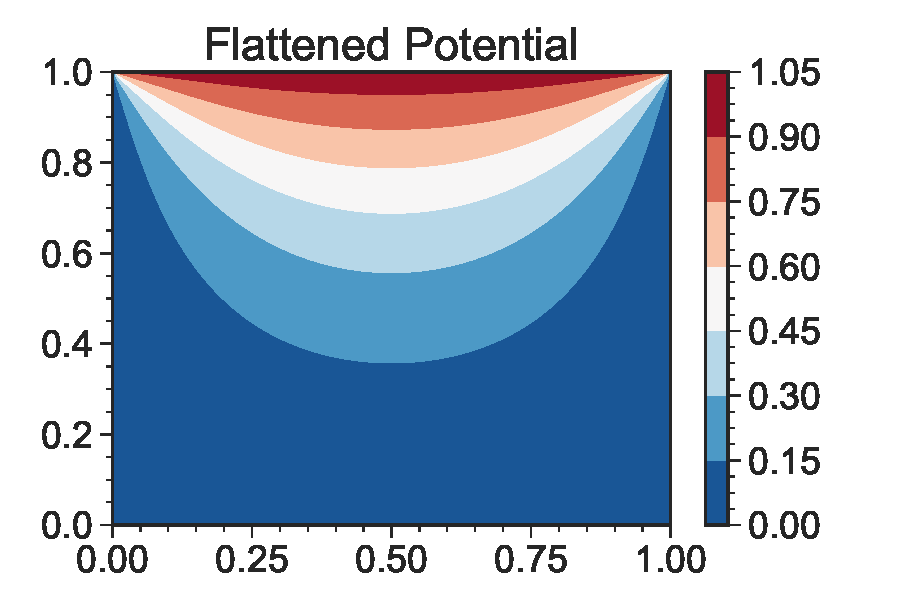
\includegraphics[width=0.3\textwidth]{Images/Fig:Countour-plot/4-contour.pdf}
        }%
        \hspace{1em}
        \subfigure[Contour plot number 5]{%
            \label{fig:Contour_5}
            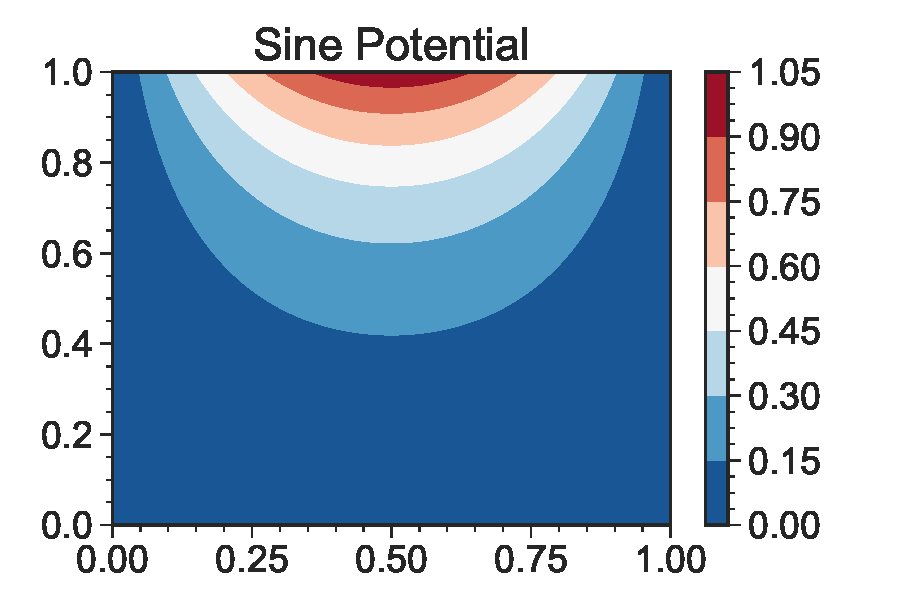
\includegraphics[width=0.3\textwidth]{Images/Fig:Countour-plot/5-contour.pdf}
        }%
        \hspace{1em}
        \subfigure[Contour plot number 6]{%
            \label{fig:Contour_6}
            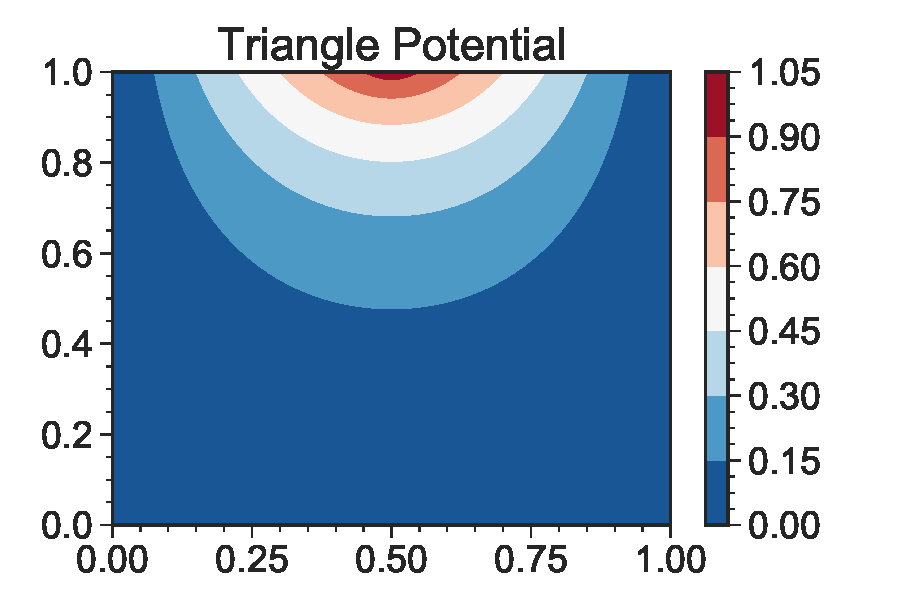
\includegraphics[width=0.3\textwidth]{Images/Fig:Countour-plot/6-contour.pdf}
        }%
%
    \caption{%
        Contour plots for different potentials $V_0(x)$, along the line $y=1$
     }%
   \label{fig:Countour-plot}
\end{figure*}                     % Change this to another line to move big figures.
\section{Messa a fuoco}
Prima di procedere con gli esperimenti è stato necessario mettere a fuoco il telescopio. Dopo averlo puntato dalla finestra del laboratorio verso un punto di riferimento abbastanza lontano, abbiamo calibrato l'oggetto in modo da avere simultaneamente nitidi la croce di puntamento e il punto di riferimento stesso.
Poichè non era possibile bloccare la componente del telescopio, determinati movimenti dello spettrometro hanno più volte modificato la messa a fuoco, rendendo necessaria la ricalibrazione dello strumento più volte durante l'esperienza.

\section{Studio attraverso il reticolo}
Quando della luce incide perpendicolarmente su un reticolo di diffrazione, si viene a creare una figura di interferenza simmetrica rispetto alla direzione di incidenza. La posizione dei punti di interferenza costruttiva (detti massimi) segue la legge \ref{rifrazione}. La luce però non era perfettamente incidente, è dunque possibile considerare l'angolo $\alpha$ di incidenza e scrivere
$$
\sin(\vartheta -\alpha)=n\dfrac{\lambda}{d}
$$
Misurando gli angoli che compaiono in questa relazione, è possibile stimare il passo del reticolo oppure il suo reciproco, di cui in questo caso si conosce il valore con precisione assoluta.
\subsection{Raccolta e analisi dati}
Per svolgere l'esperienza sono stati utilizzati reticoli diversa densità di fenditure, precisamente $300$, $600$ e $1200$ fenditure per millimetro (questi valori corrispondono all'inverso del passo del reticolo).

Per ognuno di essi è stato necessario calibare lo spettrometro in modo che gli angoli dei massimi dello stesso ordine fossero alla stessa distanza angolare dal riferimento $\vartheta_0=\ang{63}\,35'$ nel limite di incertezze sperimentali. La seguente tabella riassume le misure di calibrazione
\begin{table}[h!]
    \centering
    \begin{tabular}{cc}
    \toprule
         Reticolo & $\vartheta_{max}$ (dx/sx)$-\vartheta_0$ \\
         \midrule
         300 & \ang{32}\,30'\\
             & -\ang{32}\,30'\\
        \midrule
         600 &  \ang{46}\,0'\\
          &-\ang{45}\,17'\\
        \midrule
        1200 & \ang{45}\,10'\\
        & -\ang{45}\,2'\\
    \bottomrule
    \end{tabular}
    \caption{}
    \label{tab:my_label}
\end{table}
Dopo questa operazione abbiao misurato gli angoli dei massimi di interferenza meglio individuabili. La seguente tabella mostra i dati raccolti in questa fase
\begin{table}[h!]
    \centering
    \begin{tabular}{cccc}
    \toprule
    Reticolo & $\ang{1}$ ordine & $\ang{2}$ ordine & $\ang{3}$ ordine \\
    \midrule
    300     & \ang{73}\,48’ & \ang{84}\,38'&\ang{96}\,5'\\
    \midrule
    600     &\ang{84}\,32' & \ang{109}\,35' & \\
    \midrule
    1200 & \ang{108}\,35' & &\\
    \bottomrule
    \end{tabular}
    \caption{}
    \label{tab:my_label}
\end{table}
\subsection{Correzione sull'angolo}
La non perpendicolarità della luce incidente può essere corretta introducento l'angolo $\alpha$ il cui valore viene ricavato da considerazioni ottico geometriche da cui si giunge alla seguente relazione
\begin{equation}
    \tan\alpha=\dfrac{\sin\theta_{+}+\sin\theta_{-}}{2-\cos\theta_{+}-\cos\theta_{-}}
\end{equation}
dove $\theta_\pm$ sono gli angoli, a destra e a sinistra, a cui si trovano i massimi della figura di interferenza. Da questa relazione può essere ricavata l'incertezza relativa a questa grandezza che si trova essere
\begin{equation}
\sigma_{\alpha}^{2}=\frac{\left(2 \cos \theta_{+}-\cos \left(\theta_{+}-\theta_{-}\right)-1\right)^{2}+\left(2 \cos \theta_{-}-\cos \left(\theta_{+}-\theta_{-}\right)-1\right)^{2}}{\left(1+\tan ^{2} \alpha\right)^{2}\left(2-\cos \theta_{+}-\cos \theta_{-}\right)^{4}} \sigma_{\theta}^{2}
\end{equation}
La seguente tabella riassume i risultati raccolti
\begin{table}[h!]
    \centering
    \begin{tabular}{ccc}
    \toprule
    Reticolo & $\alpha$ & $\sigma_\alpha$\\
    \midrule
    300     &0' &5' \\
    \midrule
    600     &50' &2'\\
    \midrule
    1200 & 7' & 2' \\
    \bottomrule
    
    \end{tabular}
    \caption{}
    \label{tab:my_label}
\end{table}
\subsection{Verifica della legge di diffrazione \label{paragrafo 3}}
\begin{figure}[h!]
    \centering
    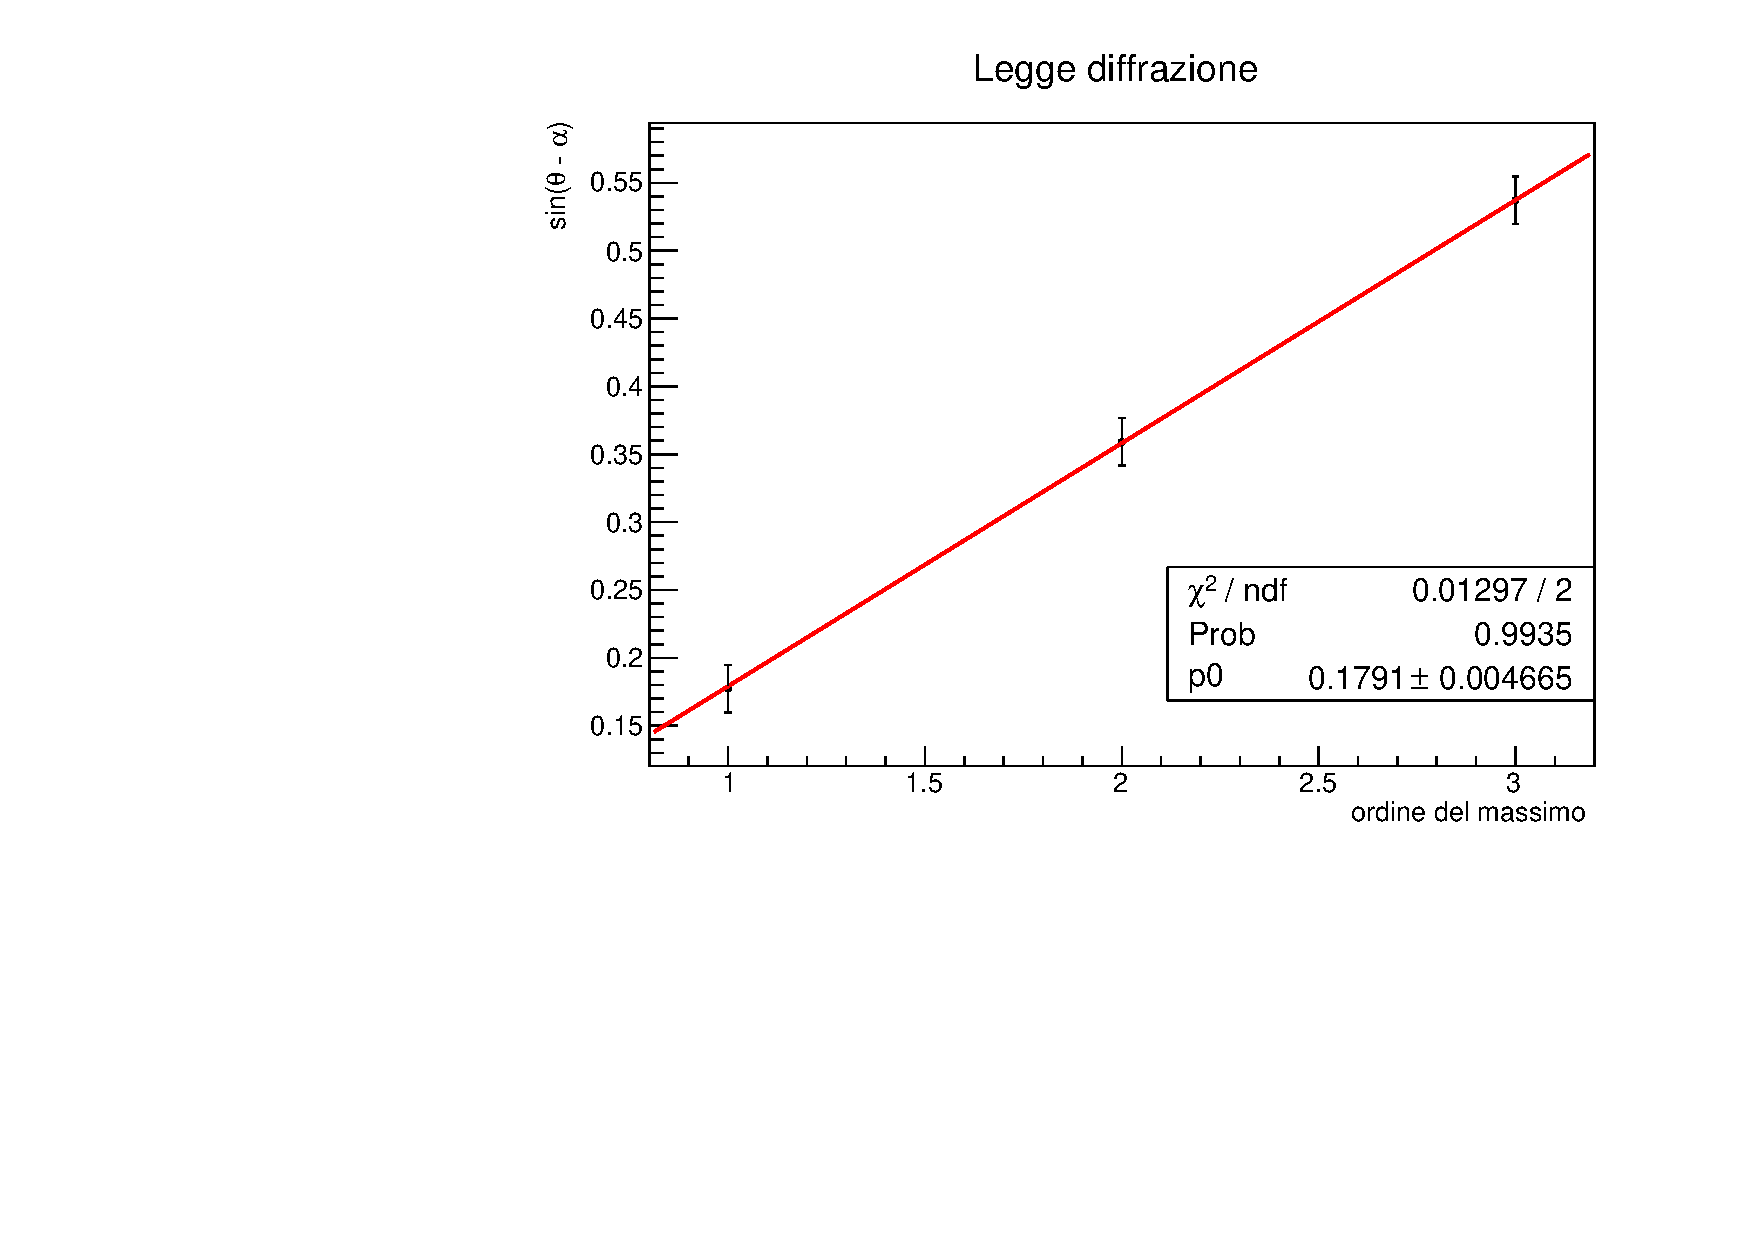
\includegraphics[scale=.6]{Immagini/legge diffrazione.pdf}
    \caption{}
    \label{fit rifrazione}
\end{figure}

Siccome utilizzando il reticolo da $300\,\frac{\text{fend.}}{\text{mm}}$ è possibile ricavare massimi di tre ordini differenti, la stima del suo passo può essere effettuata interpolando l'equazione
$$
\sin(\vartheta-\alpha)=n\dfrac{\lambda}{d}
$$
In questo modo si verifica anche la legge stessa. Chiamato $\beta=\vartheta-\alpha$ l'angolo effettivo del massimo rispetto alla normale del reticolo, si può dire che 
$$
\sigma^2_\beta = \sigma_\alpha^2+\sigma_\vartheta^2
$$
per poi effettuare il fit riportato nella Fig. \ref{fit rifrazione}. Da tale interpolazione si stima il valore caratteristico del reticolo dividendo per $\lambda$
$$
\dfrac{1}{d}=303,8\pm 0,5 \frac{\text{fend.}}{\text{mm}}
$$
Il valore ricavato di $1/d$ non è compatibile con il valore atteso di $300\,\frac{\text{fend.}}{\text{mm}}$ in quanto eseguendo il $t-$test di Student si trova che 
$$
t_s=\dfrac{\hat{\vartheta}-\vartheta_t}{\sigma_\vartheta}=7,6
$$

Questo fa presumere che la legge di diffrazione sia esatta (i dati sperimentali seguono effettivamente una proporzionalità lineare), ma che ci sia un errore nella stima del valore cercato. L’ipotesi più attendibile riguarda un errore nella stima di $\alpha$: dato che una sua variazione di pochi primi comporta un’importante variazione dei risultati, e dato che il supporto del reticolo non era vincolato in modo rigido ma libero di muoversi, si può supporre che nell’atto di misurazione degli angoli tale reticolo si sia leggermente spostato.
\subsubsection{Altri reticoli}
Siccome per gli altri reticoli non disponevamo di sufficienti misure per effettuare un'interpolazione affidabile abbiamo proceduto sitmando i parametri in maniera diretta
$$
\frac{1}{d}=\frac{1}{n \lambda} \sin (\theta-\alpha)
$$
$$
\sigma_{\frac{1}{d}}=\frac{1}{n \lambda} \cos (\theta-\alpha) \sqrt{\sigma_{\theta}^{2}+\sigma_{\alpha}^{2}}
$$
I risultati sono raccolti nella seguente tabella
\begin{table}[h!]
    \centering
    \begin{tabular}{ccc}
    \toprule
    Reticolo $(\frac{\text{fend.}}{\text{mm}})$ & $1/d$ $(\frac{\text{fend.}}{\text{mm}})$ & $\sigma_{\frac{1}{d}}$ $(\frac{\text{fend.}}{\text{mm}})$\\
    \midrule
         600 & 599,2 & 0,4 \\
         1200 &  1200,3 & 0,8\\
    \bottomrule
    \end{tabular}
    \caption{}
    \label{tab:my_label}
\end{table}
\\

In questo caso i valori sono accettabilmente compatibili con quelli attesi e ci permette di confermare la validità della legge di diffrazione, a discapito dell’errata stima fatta in precedenza.
\section{Discussione errori}
\label{discussione errori}
L'errore associato ad ogni misura è stato generato tramite un algoritmo per la generazione di numeri pseudocasuali. Infatti, eseguendo una misura del segnale senza elementi circuitali inseriti, si osserva che è sempre presente un segnale di disturbo che quindi va ad intaccare ogni misurazione variando l'intensità del segnale misurato.

Siccome è presente in ogni misurazione abbiamo ritenuto plausibile considerarlo come la principale fonte di errore, inoltre a questa fonte si deve aggiungere l'errore sistematico intrinseco dello strumento. Tale errore è stato valutato come la sensibilità dello strumento. Un ulteriore elemento a favore di questa ipotesi è che le misure sono state raccolte direttamente dallo strumento tramite una chiavetta USB per cui, a meno di errori dovuti a malfunzionamenti interni della strumentazione impossibili da identificare, possibili fonti esterne di errore sono da scartare. 

Analizzando il segnale di disturbo si è notata la presenza di valori misurati di tensione distribuiti in maniera casuale. Per tale ragione si è utilizzato un algoritmo di generazione di numeri pseudocasuali distribuiti secondo una \textit{pdf} gaussiana.

La scelta della \textit{pdf} è motivata dal fatto che i valori di tensione osservati erano meno densi agli estremi dell'intervallo mentre la densità aumentava gradualmente spostandosi nel centro dello stesso.


\section{Conclusioni}
Lo scopo di questa esperienza è stato quello di studiare e verficare relazioni e leggi riguardanti resistenze e diodi. In primo luogo è stata condotta una verifica sulle due configurazioni, quella con il voltmetro e quella con l'amperometro, al fine di analizzare i loro comportamenti rispetto alle configurazioni ideali. Per l'amperometro i risultati ottenuti risultano congruenti con quelli aspettati, cosa che invece non accade con il voltmetro. Crediamo che la causa di ciò possa essere dovuta a due principali fattori. In primis riteniamo possibile che la resistenza scelta, la quale era necessario fosse confrontabile con quella del voltmetro, potrebbe non essere stata tale e che, quindi, l'errore sull'ordine di grandezza potrebbe essere stato causato da quello. Come seconda fonte di errore riconduciamo il fatto che, per identificare le resistenze, ci siamo serviti del tool online menzionato nell'introduzione, i cui valori potrebbero non corrispondere a quelli reali, inserendo quindi un possibile errore sistematico nei nostri risultati. A causa di tale incongruenza, in esperienze che fornivano la possibilità di scegliere la configurazione, abbiamo sempre preferito utilizzare quella con l'amperometro. Lo studio sulla relazione evidenziata da Ohm risulta corretta, nonostante il $\chi^2$ risulti molto bassa. La causa più probabile di questo fenomeno potrebbe essere ricercata in una sottostima degli errori, dovuta al nostro modo di identificare i valori delle resistenze. Nonostante questa possibile fonte di errore, lo studio sul partitore resistivo ha portato risultati congruenti rispetto al nostro studio teorico riguardo alle relazioni sulle resistenze. Infine, anche l'analisi sul diodo risulta congruente rispetto alla relazione ipotizzata, con un $\chi^2$ ridotto di circa 0.82. Riteniamo che l'esperimento potrebbe essere riprodotto con risultati più soddisfacenti se si procedesse a misurare le resistenze in maniera differente. 
%\clearpage                                     % Sometimes you want the rest on separate pages.
                % Comment out to exclude the Acknowledgements section

%%%%%%%%%%%%%%%%%%%%%%%%%%%%%%%%%%%%%%%%

% Bibliography
%--------------------


\clearpage                                     % Sometimes it is useful to have appendix on separate page.
%\onecolumn                                     % If you want 1 column for appendix.
\appendix
% Delete the text and write Appendix here (not required, can be omitted):
% Comment out ' \appendix
% Delete the text and write Appendix here (not required, can be omitted):
% Comment out ' \appendix
% Delete the text and write Appendix here (not required, can be omitted):
% Comment out ' \input{Text/Appendix} ' to remove this section.
%------------------------------------
 ' to remove this section.
%------------------------------------
 ' to remove this section.
%------------------------------------
                           % Comment out to exclude appendix

\end{document}

% Notes on Copyright:
%--------------------

% Feel free to use this template as you like.
% I do not require users to give me credit for
% the use of this template, unless you share
% a verbatim (word for word) LaTeX code copy
% on the internet.

% The author may or may not release a new 
% update/ new version of this template.